\documentclass{article}
\usepackage{iclr2027_conference}
\usepackage{newtxtext}
\usepackage{amsmath,amssymb,amsthm}
\usepackage{booktabs}
\usepackage{float}
\usepackage{graphicx}
\usepackage{microtype}
\usepackage{url}
\usepackage{hyperref}
\hypersetup{colorlinks=true,linkcolor=blue,citecolor=blue,urlcolor=blue}

\newtheorem{proposition}{Proposition}
\newcommand{\Rcons}{R_{\mathrm{cons}}}
\newcommand{\dparam}{\Delta_{\mathrm{param}}}
\newcommand{\dhard}{\Delta_{\mathrm{hard}}}
\newcommand{\Ipath}{I_{\mathrm{path}}}
\newcommand{\phiP}{\phi_{\mathrm{param}}}
\newcommand{\phiE}{\phi_{\mathrm{enforce}}}
\newcommand{\FactorBenchmark}{pdebench\_advection\_beta0.4\_fno\_factorial\_v1}
\newcommand{\FactorRecords}{150}
\newcommand{\FactorPrimaryCase}{ood\_r512}
\newcommand{\FactorPrimaryHorizon}{16}
\newcommand{\FactorAZero}{0.03373}
\newcommand{\FactorRZero}{0.03219}
\newcommand{\FactorAOne}{0.03372}
\newcommand{\FactorROne}{0.03029}
\newcommand{\FactorProjected}{0.03375}
\newcommand{\FactorInteraction}{-0.00189}
\newcommand{\FactorInteractionLow}{-0.00373}
\newcommand{\FactorInteractionHigh}{-0.00025}
\newcommand{\FactorInteractionLowNinety}{-0.00339}
\newcommand{\FactorInteractionHighNinety}{-0.00051}
\newcommand{\FactorSesoi}{0.00322}
\newcommand{\FactorClassification}{statistical non-additivity below/crossing the SESOI}
\newcommand{\FactorHolmSignificantCells}{0}
\newcommand{\FactorMaterialCells}{0}
\newcommand{\FactorSmallerStatisticalCells}{4}
\newcommand{\FactorAdditiveCells}{5}
\newcommand{\FactorUnresolvedCells}{3}
\newcommand{\FactorPZero}{0.00154}
\newcommand{\FactorPZeroLow}{0.00080}
\newcommand{\FactorPZeroHigh}{0.00231}
\newcommand{\FactorPOne}{0.00343}
\newcommand{\FactorPOneLow}{0.00195}
\newcommand{\FactorPOneHigh}{0.00531}
\newcommand{\FactorEAbsolute}{1.274e-05}
\newcommand{\FactorEAbsoluteLow}{-0.00147}
\newcommand{\FactorEAbsoluteHigh}{0.00140}
\newcommand{\FactorEResidual}{0.00190}
\newcommand{\FactorEResidualLow}{0.00120}
\newcommand{\FactorEResidualHigh}{0.00264}
\newcommand{\FactorPhiParameterization}{0.00248}
\newcommand{\FactorPhiParameterizationLow}{0.00163}
\newcommand{\FactorPhiParameterizationHigh}{0.00357}
\newcommand{\FactorPhiEnforcement}{0.00096}
\newcommand{\FactorPhiEnforcementLow}{0.00023}
\newcommand{\FactorPhiEnforcementHigh}{0.00167}
\newcommand{\FactorProjectionMinusHardAbsolute}{3.899e-05}
\newcommand{\FactorProjectionMinusHardAbsoluteLow}{-0.00145}
\newcommand{\FactorProjectionMinusHardAbsoluteHigh}{0.00140}

\newcommand{\CubeCoreRecords}{150}
\newcommand{\CubeDerivedRecords}{90}
\newcommand{\CubeCheckpoints}{120}
\newcommand{\CubePrimaryCase}{ood\_r512}
\newcommand{\CubePrimaryHorizon}{16}
\newcommand{\CubeJ}{0.22974}
\newcommand{\CubeJLow}{0.19644}
\newcommand{\CubeJHigh}{0.26345}
\newcommand{\CubeSesoi}{0.00322}
\newcommand{\CubeJOverSesoi}{71.4}
\newcommand{\CubeClassification}{material non-additivity}
\newcommand{\CubeHolmP}{0.00012}
\newcommand{\CubeHolmSignificantCells}{9}
\newcommand{\CubeMaterialCells}{9}
\newcommand{\CubeSmallerStatisticalCells}{1}
\newcommand{\CubeAdditiveCells}{2}
\newcommand{\CubeUnresolvedCells}{0}
\newcommand{\CubeAZeroZero}{0.03373}
\newcommand{\CubeRZeroZero}{0.03219}
\newcommand{\CubeAZeroOne}{0.03375}
\newcommand{\CubeRZeroOne}{0.03218}
\newcommand{\CubeAOneZero}{0.36627}
\newcommand{\CubeROneZero}{0.59262}
\newcommand{\CubeAOneOne}{0.03372}
\newcommand{\CubeROneOne}{0.03029}
\newcommand{\CubeIBundle}{-0.00189}
\newcommand{\CubeIBundleLow}{-0.00375}
\newcommand{\CubeIBundleHigh}{-0.00025}
\newcommand{\CubeTZero}{0.22789}
\newcommand{\CubeTZeroLow}{0.19450}
\newcommand{\CubeTZeroHigh}{0.26127}
\newcommand{\CubeTOne}{-0.00186}
\newcommand{\CubeTOneLow}{-0.00371}
\newcommand{\CubeTOneHigh}{-0.00023}
\newcommand{\CubeEZero}{-3.456e-05}
\newcommand{\CubeEZeroLow}{-0.00011}
\newcommand{\CubeEZeroHigh}{2.946e-05}
\newcommand{\CubeEOne}{-0.22978}
\newcommand{\CubeEOneLow}{-0.26339}
\newcommand{\CubeEOneHigh}{-0.19629}
\newcommand{\CubeJEffect}{0.22974}
\newcommand{\CubeJEffectLow}{0.19644}
\newcommand{\CubeJEffectHigh}{0.26345}
\newcommand{\CubePhiTrain}{0.11302}
\newcommand{\CubePhiTrainLow}{0.09634}
\newcommand{\CubePhiTrainHigh}{0.12975}
\newcommand{\CubePhiInfer}{-0.11491}
\newcommand{\CubePhiInferLow}{-0.13166}
\newcommand{\CubePhiInferHigh}{-0.09818}
\newcommand{\CubeGradientRecords}{60}
\newcommand{\CubeOneStepInteraction}{0.00015}
\newcommand{\CubeOneStepInteractionLow}{0.00012}
\newcommand{\CubeOneStepInteractionHigh}{0.00019}
\newcommand{\CubeFinalTrainingInteraction}{-0.00186}
\newcommand{\CubeFinalTrainingInteractionLow}{-0.00370}
\newcommand{\CubeFinalTrainingInteractionHigh}{-0.00022}
\newcommand{\CubeMechanismRho}{0.062}
\newcommand{\CubeMechanismRhoLow}{-0.297}
\newcommand{\CubeMechanismRhoHigh}{0.398}
\newcommand{\CubeMechanismClassification}{not supported}

\newcommand{\SWECoreRecords}{150}
\newcommand{\SWEDerivedRecords}{90}
\newcommand{\SWECheckpoints}{120}
\newcommand{\SWEPrimaryCase}{ood\_r128}
\newcommand{\SWEPrimaryHorizon}{16}
\newcommand{\SWEJ}{-86.69343}
\newcommand{\SWEJLow}{-107.65055}
\newcommand{\SWEJHigh}{-66.68345}
\newcommand{\SWESesoi}{0.01501}
\newcommand{\SWEJOverSesoi}{5777.2}
\newcommand{\SWEClassification}{material non-additivity}
\newcommand{\SWEHolmP}{8.000e-05}
\newcommand{\SWEMaterialCells}{6}
\newcommand{\SWESmallerStatisticalCells}{0}
\newcommand{\SWEAdditiveCells}{2}
\newcommand{\SWEUnresolvedCells}{0}
\newcommand{\SWETradeoffCase}{ood\_r128}
\newcommand{\SWETradeoffHorizon}{31}
\newcommand{\SWETradeoffClassification}{resolved conservation--positivity synergy}
\newcommand{\SWEAZeroZero}{0.12461}
\newcommand{\SWERZeroZero}{0.15006}
\newcommand{\SWEAZeroOne}{0.11774}
\newcommand{\SWERZeroOne}{0.15006}
\newcommand{\SWEAOneZero}{86.79537}
\newcommand{\SWEROneZero}{0.15006}
\newcommand{\SWEAOneOne}{0.09507}
\newcommand{\SWEROneOne}{0.15006}
\newcommand{\SWEIBundle}{0.02954}
\newcommand{\SWEIBundleLow}{0.01529}
\newcommand{\SWEIBundleHigh}{0.04375}
\newcommand{\SWETZero}{-86.67076}
\newcommand{\SWETZeroLow}{-107.64014}
\newcommand{\SWETZeroHigh}{-66.69689}
\newcommand{\SWETOne}{0.02267}
\newcommand{\SWETOneLow}{0.01039}
\newcommand{\SWETOneHigh}{0.03456}
\newcommand{\SWEEZero}{0.00687}
\newcommand{\SWEEZeroLow}{0.00342}
\newcommand{\SWEEZeroHigh}{0.01065}
\newcommand{\SWEEOne}{86.70030}
\newcommand{\SWEEOneLow}{66.54583}
\newcommand{\SWEEOneHigh}{107.70683}
\newcommand{\SWEPhiTrain}{-43.32405}
\newcommand{\SWEPhiTrainLow}{-53.84650}
\newcommand{\SWEPhiTrainHigh}{-33.19291}
\newcommand{\SWEPhiInfer}{43.35358}
\newcommand{\SWEPhiInferLow}{33.32056}
\newcommand{\SWEPhiInferHigh}{53.97078}
\newcommand{\SWETradeoffConservation}{0.46656}
\newcommand{\SWETradeoffConservationLow}{0.35540}
\newcommand{\SWETradeoffConservationHigh}{0.58242}
\newcommand{\SWETradeoffPositivity}{9.864e-05}
\newcommand{\SWETradeoffPositivityLow}{3.640e-08}
\newcommand{\SWETradeoffPositivityHigh}{0.00028}
\newcommand{\SWETradeoffNegativeFraction}{0.00065}
\newcommand{\SWETradeoffNegativeFractionLow}{2.011e-06}
\newcommand{\SWETradeoffNegativeFractionHigh}{0.00169}
\newcommand{\SWETradeoffDynamics}{0.06994}
\newcommand{\SWETradeoffDynamicsLow}{0.04168}
\newcommand{\SWETradeoffDynamicsHigh}{0.10034}
\newcommand{\SWECoreInteraction}{0.02954}
\newcommand{\SWECoreInteractionLow}{0.01534}
\newcommand{\SWECoreInteractionHigh}{0.04369}
\newcommand{\SWECoreClassification}{material non-additivity}

\newcommand{\GaugeRecords}{60}
\newcommand{\GaugeCheckpoints}{120}
\newcommand{\GaugePrimaryCase}{ood\_r512}
\newcommand{\GaugeThreshold}{0.10000}
\newcommand{\GaugeClassification}{material gauge feedback}
\newcommand{\GaugeAssociationClassification}{not supported}
\newcommand{\GaugeMaxContamination}{6.549e-05}
\newcommand{\GaugeContaminationLimit}{0.00100}
\newcommand{\GaugeMaterialCases}{3}
\newcommand{\GaugeRatio}{8.68398}
\newcommand{\GaugeRatioLow}{7.91007}
\newcommand{\GaugeRatioHigh}{9.50538}
\newcommand{\GaugeRatioOverThreshold}{86.8}
\newcommand{\GaugeFeedbackRMSE}{0.17447}
\newcommand{\GaugeFeedbackRMSELow}{0.15881}
\newcommand{\GaugeFeedbackRMSEHigh}{0.19064}
\newcommand{\GaugeAbsoluteRatio}{8.20592}
\newcommand{\GaugeAbsoluteRatioLow}{6.66317}
\newcommand{\GaugeAbsoluteRatioHigh}{9.81469}
\newcommand{\GaugeResidualRatio}{9.16205}
\newcommand{\GaugeResidualRatioLow}{9.06965}
\newcommand{\GaugeResidualRatioHigh}{9.27338}
\newcommand{\GaugeAssociationRho}{0.28765}
\newcommand{\GaugeAssociationRhoLow}{-0.09679}
\newcommand{\GaugeAssociationRhoHigh}{0.62675}

\newcommand{\UNetCoreRecords}{150}
\newcommand{\UNetDerivedRecords}{90}
\newcommand{\UNetCheckpoints}{120}
\newcommand{\UNetJ}{-0.08415}
\newcommand{\UNetJLow}{-0.26665}
\newcommand{\UNetJHigh}{0.13334}
\newcommand{\UNetSesoi}{0.14751}
\newcommand{\UNetJOverSesoi}{0.6}
\newcommand{\UNetClassification}{unresolved}
\newcommand{\UNetHolmP}{1.00000}
\newcommand{\UNetMaterialCells}{3}
\newcommand{\UNetSmallerStatisticalCells}{6}
\newcommand{\UNetAdditiveCells}{1}
\newcommand{\UNetUnresolvedCells}{2}
\newcommand{\UNetAdmission}{did not pass}
\newcommand{\UNetCoreSHA}{ae0dda1c95e5}
\newcommand{\UNetCoreAnalysisSHA}{6e3252b5a1d3}
\newcommand{\UNetLockSHA}{e7d43d3d3ce9}
\newcommand{\UNetCubeSHA}{01a23a0b77ff}
\newcommand{\UNetCubeAnalysisSHA}{0e2ad4bdf6f9}
\newcommand{\UNetIBundle}{0.10234}
\newcommand{\UNetIBundleLow}{0.00507}
\newcommand{\UNetIBundleHigh}{0.19831}
\newcommand{\UNetTZero}{0.02382}
\newcommand{\UNetTZeroLow}{-0.19196}
\newcommand{\UNetTZeroHigh}{0.28132}
\newcommand{\UNetTOne}{0.10797}
\newcommand{\UNetTOneLow}{0.01193}
\newcommand{\UNetTOneHigh}{0.20349}
\newcommand{\UNetEZero}{-0.00562}
\newcommand{\UNetEZeroLow}{-0.01160}
\newcommand{\UNetEZeroHigh}{-0.00047}
\newcommand{\UNetEOne}{0.07853}
\newcommand{\UNetEOneLow}{-0.14004}
\newcommand{\UNetEOneHigh}{0.26256}
\newcommand{\UNetPhiTrain}{0.06589}
\newcommand{\UNetPhiTrainLow}{-0.07577}
\newcommand{\UNetPhiTrainHigh}{0.22755}
\newcommand{\UNetPhiInfer}{0.03645}
\newcommand{\UNetPhiInferLow}{-0.07036}
\newcommand{\UNetPhiInferHigh}{0.12614}
\newcommand{\UNetAZeroZero}{0.86332}
\newcommand{\UNetRZeroZero}{1.47514}
\newcommand{\UNetAZeroOne}{0.86423}
\newcommand{\UNetRZeroOne}{1.47043}
\newcommand{\UNetAOneZero}{0.82239}
\newcommand{\UNetROneZero}{1.45803}
\newcommand{\UNetAOneOne}{0.83205}
\newcommand{\UNetROneOne}{1.54622}

\newcommand{\SyntheticSystems}{8}
\newcommand{\SyntheticParameterizationNonzero}{8}
\newcommand{\SyntheticParameterizationHolm}{8}
\newcommand{\SyntheticResidualFavored}{6}
\newcommand{\SyntheticEquivalent}{6}
\newcommand{\SyntheticFullPass}{1}


\title{When Are Exact Conservation Layers Plug-and-Play?\\
Identifying Training--Inference Path Dependence\\
in Neural PDE Surrogates}
\author{Anonymous authors}

% Keep commented for anonymous submission.
% \iclrfinalcopy

\begin{document}
\maketitle

\begin{abstract}
Exact conservation layers are often treated as modular post-processors, but in autoregressive
surrogates projection during training changes the learned representation and projection during
inference changes future inputs. We separate these interventions with an eight-cell
output-coordinate-by-training-by-inference cube and prove that projected training leaves the raw
invariant channel gauge-nonidentifiable. In a prospectively frozen, 30-seed PDEBench Advection
experiment, a small ordinary bundled interaction ($\FactorInteraction$) conceals a three-way
interaction of $\CubeJ$ [$\CubeJLow$, $\CubeJHigh$], material in \CubeMaterialCells/12 mandatory
resolution--horizon cells. Opposite-signed training and inference path credits cancel, and damage
from removing projection appears only after autoregressive feedback. An independently frozen
30-seed 2D shallow-water replication gives $J=\SWEJ$ [\SWEJLow, \SWEJHigh], material in
\SWEMaterialCells/8 cells, while projection jointly improves conservation, conserving RMSE, and
positivity. A separately registered larger U-Net transfer does not meet its gate:
$J=\UNetJ$ [\UNetJLow, \UNetJHigh] is unresolved and only \UNetMaterialCells/12 cells are
material. A direct same-checkpoint input-gauge intervention yields an OOD
feedback-to-baseline ratio of \GaugeRatio{} [\GaugeRatioLow, \GaugeRatioHigh], above the frozen
0.10 threshold at all resolutions. Its seed-level association with final damage, like a local
gradient association, remains unsupported. Exact enforcement can therefore become non-detachable:
projected training can identify the deployed predictor while leaving its raw invariant component
undefined in the tested FNOs, but the U-Net boundary precludes an architecture-general claim.
\end{abstract}

\section{Introduction}

Learned simulators can achieve low average error while violating identities that the modeled
system satisfies exactly. Architectural constraint layers, output projection, probabilistic
conditioning, and physics penalties address this problem in climate emulation, PDE surrogate
modeling, and neural operators \citep{beucler2021,hansen2023,harder2023,liu2024clawno}. Exact
enforcement has an unambiguous benefit: every returned state belongs to the admissible set. A
different claim---that the constraint itself improved predictive accuracy or out-of-distribution
(OOD) generalization---requires a controlled attribution design.

That control is easy to miss. Autoregressive simulators may predict an absolute next state
$f_\theta(x_t)$ or an update $x_t+g_\theta(x_t)$. Exact conservation is naturally implemented by
projecting the update into the invariant tangent space. Comparing this hard residual model only
with an unconstrained absolute-output model changes two factors at once: output parameterization
and enforcement. Residual updates are themselves a strong inductive bias in learned simulation
\citep{pfaff2021}. A favorable comparison therefore does not identify which factor deserves
credit.

We study attribution rather than proposing another enforcement operator. The trained design
crosses absolute/residual outputs with free/hard training; toggling projection on each locked
checkpoint completes an eight-cell cube without optimization. This also exposes that projected
training identifies raw outputs only modulo the invariant direction: a checkpoint may be accurate
with its projector and unstable without it despite one-step conserving equivalence. Thus
``plug-and-play'' means safe same-checkpoint composition through rollout, not software
compatibility or exact constraint satisfaction.

Our contributions are:
\begin{itemize}
  \item an eight-cell intervention design that separately identifies output coordinate, training
  enforcement, inference enforcement, and their three-way path dependence;
  \item a projection-gauge non-identifiability result and a direct same-checkpoint intervention
  showing that an invariant-direction input change transfers materially into conserving dynamics;
  \item prospectively frozen 30-seed Advection and independently frozen 30-seed 2D shallow-water
  FNO evidence, plus a registered larger U-Net transfer that does not pass its gate; and
  \item orthogonal error and tangent-kernel analyses, including a frozen local mechanism test whose
  unsupported final association bounds rather than embellishes the explanation.
\end{itemize}

\section{Related work}

\paragraph{Encoding physical constraints.}
Hard constraints enforce analytic identities through architectures, invariant operators,
projection, probabilistic correction, or learned correction
\citep{beucler2021,richterpowell2022,liu2023ino,liu2024clawno,hansen2023,mouli2024,
zhang2023concernet,harder2023,tanaka2025,liu2025adaptive}. Most directly,
\citet{duruisseaux2024} compare an unconstrained FNO, post-hoc projection, constraint finetuning,
and projected training; a contemporaneous submission ablates tangent-space projection and residual
guidance \citep{anonymous2026pmfm}. These establish end-to-end feasibility and accuracy, but do not
remove projection from the same constrained checkpoint, cross output coordinates, and follow that
same-weight intervention through autoregressive feedback. Our target is this
training-by-deployment interaction, not a replacement enforcement architecture.

\paragraph{Gradient interaction in physics learning.}
Composite PINN objectives can produce severe gradient-scale imbalance or directional conflict;
adaptive scaling, dual-cone updates, and second-order preconditioning have been proposed to address
these optimization pathologies \citep{yao2023multiadam,hwang2024dcgd,wang2025gradient}. Our
mechanism question is narrower and structurally different: the two squared-error channels are
orthogonal in output space, but a shared neural operator can map them to non-orthogonal parameter
gradients. We do not propose a new optimizer. We use their alignment and an exact free-versus-hard
one-step intervention to test whether this parameter-space coupling helps explain attribution.

\paragraph{Neural PDE evaluation.}
Fourier neural operators (FNOs) learn mappings between function spaces and support evaluation at
unseen discretizations \citep{li2021fno}. PDEBench provides standardized time-dependent PDE data,
baselines, and metrics, including conservation-aware diagnostics \citep{pdebench}. Our experiments
use its public Advection and two-dimensional shallow-water data, but change the evaluation
question: rather than ranking a new operator, we estimate paired effects of parameterization and
enforcement under the same locked weights.

\section{A matched attribution audit}
\label{sec:audit}

\subsection{Linear invariant and error channels}

Let $x\in\mathbb{R}^n$ be the last observed state and $y$ the true next state. For a nonzero
$a\in\mathbb{R}^n$, the linear invariant is $a^\top y=a^\top x$. Define the orthogonal projectors
\begin{equation}
  P=\frac{aa^\top}{\lVert a\rVert_2^2},\qquad Q=I-P.
\end{equation}
For prediction $\hat y$ and error $e=\hat y-y$, $Pe$ is the invariant-violating channel and $Qe$
is the conserving channel. We report conserving RMSE, $\Rcons$, from $Qe$. This metric deliberately
does not reward a method merely for removing the mean error; total squared error decomposes as
$\lVert e\rVert_2^2=\lVert Qe\rVert_2^2+\lVert Pe\rVert_2^2$.

The least-squares projection of an absolute prediction onto the affine invariant set is
\begin{equation}
  \Pi_x(\hat y)=\hat y-P(\hat y-x).
\end{equation}

\begin{proposition}[Projection decoupling]
\label{prop:decoupling}
If $a^\top y=a^\top x$, then
$\Pi_x(\hat y)-y=Q(\hat y-y)$. Consequently, projection removes the violating channel exactly and
leaves the conserving-channel error unchanged.
\end{proposition}

The proof is in Appendix~\ref{app:proof}. In the experiment, the post-hoc projection of the trained
free model is therefore an implementation control, not an independent learned baseline.

\begin{proposition}[Projected-training gauge]
\label{prop:gauge}
For any raw predictor $z(x)$ and scalar function $\alpha(x)$,
$\Pi_x(z(x)+\alpha(x)a)=\Pi_x(z(x))$. Hence, in any hypothesis class closed under this
transformation, a loss applied only after projection cannot identify the raw predictor's
invariant-channel component. Removing the projector from a hard-trained checkpoint selects an
unidentified representative of the same deployed predictor.
\end{proposition}

The proof is in Appendix~\ref{app:gauge}. Proposition~\ref{prop:decoupling} still makes the
projected and unprojected predictions agree in conserving error for the same one-step input.
For our FNO, the bias in its final pointwise map realizes at least every constant shift $\alpha a$,
so the closure condition is not merely an unrestricted-function abstraction.
Autoregressive equivalence does not follow: an unprojected invariant-channel error changes the next
input, where the network's conserving response can differ. This yields a falsifiable signature of
gauge exposure followed by state feedback---one-step equality followed by multi-step divergence.

Exact satisfaction of one invariant need not imply physical admissibility under another
constraint. This distinction matters for conserved nonnegative fields such as water depth. Write
$m(v)=n^{-1}\mathbf{1}^{\top}v$ for the uniform-grid mean.

\begin{proposition}[Conservation--positivity compatibility]
\label{prop:positivity}
For the uniform-mass invariant, $\Pi_x(z)=z+[m(x)-m(z)]\mathbf{1}$. If $z\geq0$, the projected
state is componentwise nonnegative if and only if
$\min_i z_i\geq m(z)-m(x)$. Hence an orthogonal mass projection can enforce conservation exactly
while introducing negative state values.
\end{proposition}

This exact criterion motivates reporting invariant drift, conserving-channel forecast error, and
admissible-set violations as three separate outcomes. In particular, clamping a projected field
would silently compose two interventions and destroy the clean training-by-inference factorial.

The fixed-prediction statement also supplies a training-time null model. Let a coordinate choice
$s\in\{A,R\}$ have base map $b_A(x)=0$ or $b_R(x)=x$, and write the learned raw map as
$z_\theta(x)$. Free and hard training have the same conserving prediction
$Q(b_s(x)+z_\theta(x))$; they differ only because the free loss also contains the violating
channel.

\begin{proposition}[Channel-separable training null]
\label{prop:training-null}
Suppose $\theta=(\theta_Q,\theta_P)$ and
$z_\theta=z_Q(\theta_Q)+z_P(\theta_P)$, where $Pz_Q=0$, $Qz_P=0$, the regularizer separates over
the two parameter blocks, and paired free and hard runs use identical minibatches,
initial $\theta_Q$, and a blockwise deterministic optimizer. Then their $\theta_Q$ iterates and
conserving predictions are identical. Consequently, exact enforcement has zero
conserving-channel training effect in that coordinate system.
\end{proposition}

The proof is in Appendix~\ref{app:training-null}. A nonzero inference-matched training credit
therefore rejects this separable-training null: training through the projector changed the
admissible prediction through shared parameters, regularization, or optimization. A nonzero
coordinate-by-training interaction makes the stronger statement that this coupling depends on
absolute versus residual output coordinates. A bundled hard-versus-free rollout contrast is not
enough for either conclusion because per-step projection also changes later inputs.

The first optimization step yields a sharper local diagnostic. Decompose the free squared loss as
$L=L_Q+L_P$ and write $g_Q=\nabla L_Q(\theta)$ and $g_P=\nabla L_P(\theta)$.

For a stacked minibatch prediction $h_\theta$, let $e=h_\theta-y$, let $J_\theta$ be its parameter
Jacobian, and let $\bar P$ and $\bar Q$ apply $P$ and $Q$ independently to every example. The
finite-width empirical tangent kernel is $K_\theta=J_\theta J_\theta^\top$
\citep{jacot2018ntk}. Take $L_Q=\tfrac12\lVert\bar Qe\rVert^2$ and
$L_P=\tfrac12\lVert\bar Pe\rVert^2$; a common normalization only rescales the step size.

\begin{proposition}[Tangent-kernel channel transfer]
\label{prop:ntk-transfer}
Let $h_\theta^{\mathrm{lin}}(\theta+u)=h_\theta+J_\theta u$. From the same parameters, take a free
gradient step $\theta_F^+=\theta-\eta(g_Q+g_P)$ and a hard step
$\theta_H^+=\theta-\eta g_Q$. Then
\begin{align}
  \bar Q\!\left[h_\theta^{\mathrm{lin}}(\theta_F^+)
  -h_\theta^{\mathrm{lin}}(\theta_H^+)\right]
  &=-\eta\,\bar QK_\theta\bar P e, \\
  \langle g_Q,g_P\rangle
  &=(\bar Qe)^\top K_\theta(\bar Pe).
  \label{eq:ntk-transfer}
\end{align}
Thus the violating-channel gradient has zero first-order effect on the conserving prediction for
every violating residual if and only if the off-diagonal channel block
$\bar QK_\theta\bar P$ vanishes.
\end{proposition}

The proof is in Appendix~\ref{app:ntk-transfer}. This identity links the global separable-training
null to a measurable local mechanism. Shared
parameters need not produce a nonzero off-diagonal block, but any nonzero block is a route by which
hard enforcement can change admissible predictions even though $P$ and $Q$ are orthogonal in
output space.

\begin{proposition}[One-step gradient coupling]
\label{prop:gradient-coupling}
If $\nabla L_Q$ is $\beta$-Lipschitz, then a gradient-descent step of size $\eta$ obeys
\begin{equation}
  L_Q\!\left(\theta-\eta(g_Q+g_P)\right)
  -L_Q\!\left(\theta-\eta g_Q\right)
  =-\eta\langle g_Q,g_P\rangle+r,
  \label{eq:gradient-coupling}
\end{equation}
where
$|r|\leq\frac{\beta\eta^2}{2}
\left(\lVert g_Q+g_P\rVert_2^2+\lVert g_Q\rVert_2^2\right)$.
\end{proposition}

The proof is in Appendix~\ref{app:gradient-coupling}. Negative gradient alignment therefore makes
removing the violating-channel gradient locally favorable for $L_Q$, up to the stated remainder;
positive alignment reverses that direction. Output coordinates can change $g_P$, providing a
testable local mechanism for the factorial interaction. Because the actual optimizer is Adam and
training is nonlinear, we prospectively record both the gradient geometry and the exact matched
one-Adam-step difference; neither is assumed to explain the final rollout interaction. This use of
gradient alignment follows the broader composite-loss diagnostic literature
\citep{hwang2024dcgd,wang2025gradient}, while the orthogonal conservation channels and matched
enforcement intervention are specific to our audit.

\subsection{Mechanisms, path dependence, and path-averaged credit}

The trained FNO body and parameter count are identical across mechanisms. With raw network output
$g_\theta(x)$, the relevant arms are
\begin{align}
  \texttt{free}:&\quad \hat y=f_\theta(x), \\
  \texttt{free\_res}:&\quad \hat y=x+g_\theta(x), \\
  \texttt{hard\_abs}:&\quad \hat y=\Pi_x(f_\theta(x)), \\
  \texttt{hard}:&\quad \hat y=x+Qg_\theta(x), \\
  \texttt{projection}:&\quad \hat y=\Pi_x(f_\theta(x)).
\end{align}
For \texttt{hard\_abs}, gradients pass through $\Pi_x$ throughout training. For
\texttt{projection}, $\theta$ is the already trained \texttt{free} parameter vector and projection
is applied only as a derived evaluation transform; there is no fifth training run.
The two confirmatory contrasts use conserving RMSE averaged over the same 30 seeds:
\begin{equation}
  \dparam=\Rcons(\texttt{free})-\Rcons(\texttt{free\_res}),\qquad
  \dhard=\Rcons(\texttt{hard})-\Rcons(\texttt{free\_res}).
\end{equation}
Positive $\dparam$ favors residual parameterization; negative $\dhard$ favors hard enforcement.
Together they give a path-specific decomposition of the bundled comparison,
$\Rcons(\texttt{free})-\Rcons(\texttt{hard})=\dparam-\dhard$. They do not estimate a fully crossed
parameterization-by-training interaction.

\begin{proposition}[Three-cell non-identification]
\label{prop:missing-cell}
Without an additivity or other structural restriction on the missing potential outcome, observing
only $Y_{A0}$, $Y_{R0}$, and $Y_{R1}$ does not identify the factorial interaction or a unique
path-averaged allocation. Infinitely many nonnegative values of the unobserved trained cell
$Y_{A1}$ preserve those three observations while giving distinct values of $\Ipath$ and the two
Shapley credits.
\end{proposition}

The proof is in Appendix~\ref{app:missing-cell}. Consequently, neither a favorable three-arm
sequence nor post-hoc projection of $A0$ can identify what training in the missing absolute-hard
cell would have done. The projection is essential as an algebraic control, but it is not that
trained intervention.

To identify that interaction, let $Y_{A0},Y_{R0},Y_{A1},Y_{R1}$ denote paired-seed conserving RMSE
for absolute versus residual coordinates ($A,R$) crossed with free versus hard enforcement
($0,1$). Define positive credits as error reductions,
\begin{align}
  P_0&=Y_{A0}-Y_{R0}, & P_1&=Y_{A1}-Y_{R1},\\
  E_A&=Y_{A0}-Y_{A1}, & E_R&=Y_{R0}-Y_{R1}.
\end{align}
The parameterization credit differs across enforcement levels by
\begin{equation}
  \Ipath=P_0-P_1=E_A-E_R=Y_{A0}-Y_{R0}-Y_{A1}+Y_{R1}.
  \label{eq:interaction}
\end{equation}
Thus $\Ipath$ is simultaneously the factorial interaction and the discrepancy between two
sequential credit-allocation paths. When it is not practically negligible, neither single path
defines a unique contribution. We then use the exact two-factor Shapley averages
\begin{equation}
  \phiP=\tfrac12(P_0+P_1),\qquad
  \phiE=\tfrac12(E_A+E_R),\qquad
  \phiP+\phiE=Y_{A0}-Y_{R1}.
  \label{eq:shapley}
\end{equation}
These are intervention credits computed from trained factorial cells, not feature-attribution
scores. They average over the two possible orders instead of choosing the more favorable path
after observing results \citep{shapley1953}.

For the factorial primary cell, the smallest effect size of interest (SESOI) is
$\delta=0.1\,\overline{Y}_{R0}$. The ordered frozen classification is: \emph{material
non-additivity} if the 95\% paired-bootstrap interval for $\Ipath$ lies wholly above $+\delta$ or
below $-\delta$; \emph{smaller statistical non-additivity} if that interval excludes zero but the
first rule does not pass; \emph{practical additivity} if the 90\% interval lies wholly inside
$[-\delta,+\delta]$; and \emph{unresolved} otherwise. Thus both interaction and additivity are
falsifiable, while an interval spanning both zero and a SESOI boundary receives no positive label.
Seeds, not trajectories or rollout frames, are the inference units; each bootstrap draw resamples
the complete paired four-cell seed vector. We use 50,000 draws. Twelve secondary interaction
sign-flip tests receive Holm correction but cannot override the primary classification.

\subsection{Separating training enforcement from inference projection}

For multi-step rollouts, let $Y_{cte}$ denote conserving RMSE in coordinate $c\in\{A,R\}$, with
projector use during training $t\in\{0,1\}$ and at every inference step $e\in\{0,1\}$. The four
trained models give $Y_{A00},Y_{R00},Y_{A11},Y_{R11}$. Changing only the compatible forward map at
evaluation supplies the other four cells; all such records take zero optimizer steps. Define the
coordinate contrast $D_{te}=Y_{Ate}-Y_{Rte}$. Then
\begin{align}
  I_{\mathrm{bundle}} &=D_{00}-D_{11},\\
  T_0&=D_{00}-D_{10}, & T_1&=D_{01}-D_{11},\\
  E_0&=D_{00}-D_{01}, & E_1&=D_{10}-D_{11},\\
  J&=T_0-T_1=E_0-E_1=D_{00}-D_{10}-D_{01}+D_{11}.
\end{align}
Here $J$ is the coordinate-by-training-by-inference interaction. The path-averaged credits
\begin{equation}
  \phi_{\mathrm{train}}=\tfrac12(T_0+T_1),\qquad
  \phi_{\mathrm{infer}}=\tfrac12(E_0+E_1)
\end{equation}
obey $\phi_{\mathrm{train}}+\phi_{\mathrm{infer}}=I_{\mathrm{bundle}}$. We froze this cube while
the fresh factorial was incomplete and no metric had been accessed. Its primary cell, bootstrap,
SESOI, and ordered classification are inherited from the two-factor audit. The local gradient
diagnostic is matched to $T_1$, where both endpoints use projected inference; its association with
$I_{\mathrm{bundle}}$ is retained only as a labeled secondary analysis.

\section{PDEBench protocols}
\label{sec:protocol}

\paragraph{Data and invariant.}
We use PDEBench 1D Advection with velocity $\beta=0.4$ and periodic boundary conditions
\citep{pdebench,pdebenchdata}. The native tensor contains 10,000 trajectories, 201 used frames,
and 1024 spatial cells. The spatial mean (equivalently, uniform-grid mass) is invariant. A frozen
admission gate checks file hashes, schema, finiteness, and target-mean drift. To construct 512- and
256-cell fields without changing the invariant, we average consecutive blocks of two and four
native cells in float64 before casting to float32; point decimation was rejected prospectively
because it did not preserve the discrete mean.

Trajectories 0--255 are the external test set, 1000--8999 form the training pool, and 9000--9255
were used only for outcome-blind data preflight. Each seed samples 2,048 unique training
trajectories. Inputs are 10 frames and the target is the next frame at temporal stride five
(physical time 0.05). Models train only on 256 cells and are evaluated without retraining on ID
256 and OOD 512 and 1024 cells at autoregressive horizons $\{1,4,16,31\}$.

\paragraph{Model and optimization.}
The FNO has width 20, 12 Fourier modes, four spectral-plus-pointwise blocks, padding two, GELU
activations, and projection width 128 \citep{li2021fno}. Every trained arm uses Adam with learning
rate $10^{-3}$, weight decay $10^{-4}$, batch size 50, 200 epochs, and a StepLR decay of 0.5 at
epoch 100. There is no validation selection, early stopping, or hyperparameter search. Arms within
a seed share the sampled trajectories, minibatch order, training windows, and initial parameter
tensor. The formal factorial runs all four trained cells from identical initial tensors with fresh
seeds 3000--3029; no earlier checkpoint, seed, or record is reused. Its protocol and analysis rule
were frozen after a path-specific parent study but before seed 2999 preflight or any formal model
run. The parent study and its soft-penalty arm remain archived as historical stress tests; they do
not determine any estimate or claim here.

After observing the FNO result but before any U-Net record existed, we froze a transfer test that
changes only the model body. The two-level fully convolutional 1D U-Net
\citep{ronneberger2015unet} uses base width 20, GroupNorm, SiLU, average-pooling, transposed-convolution
upsampling, skip connections, and spatial coordinates. Data, splits, training arms, optimization,
evaluation cells, and decision rule are unchanged, with fresh paired seeds 7000--7029. Its fixed
gate requires a material primary $J$ and at least 6/12 material cells. This is neither a
capacity-matched architecture effect (FNO: 23,937 parameters; U-Net: 66,941) nor a claim that a
finite-receptive-field U-Net is a discretization-invariant operator.

Before inspecting any factorial metric, we separately froze a mechanism audit that reconstructs
each seed's exact epoch-zero first minibatch. In absolute and residual coordinates it decomposes
the full loss into $L_Q+L_P$, records $\langle g_Q,g_P\rangle$ and its cosine, and executes matched
free and hard one-step Adam updates from the identical initial tensor. Its local interaction is
the absolute-minus-residual difference between post-step free-minus-hard conserving losses. The
frozen construct-corrected primary test is the paired-seed Spearman association between that local
interaction and the inference-matched training interaction $T_1$, with a 50,000-draw 95\%
bootstrap interval. The original association with the bundled interaction remains secondary.
A non-positive or zero-crossing interval does not support the proposed local mechanism.

After the cube was complete and that gradient association was unsupported, we froze a targeted
same-checkpoint gauge intervention before any new record existed. From one ground-truth history it
computes a hard checkpoint's compatible raw state $z_1$ and projection $p_1$, appends each to an
otherwise identical history, and compares the conserving channel of the next raw prediction. The
primary per-seed estimand is this feedback RMSE divided by the projected-history branch's conserving
RMSE, averaged across coordinates at OOD 512; materiality requires its 95\% interval to lie wholly
above 0.10. The exact 60-record run crosses 30 seeds and two coordinates with zero optimization.
An initial 10-record attempt was excluded without metric access after a fixed absolute float32
identity audit rejected representational roundoff. The fresh provenance run retained the original
$10^{-6}$ floor and additionally required both a worst-case IEEE-754 bound and non-invariant
roundoff below 0.1\% of the projected baseline.

\paragraph{Prospective primary and integrity gates.}
The primary cell was fixed as OOD 512 at horizon 16; the other 11 cells were mandatory secondary
results. The core contract is exactly 150 records: 30 seeds times four trained arms plus one
zero-training projection. After its one-shot analyzer passed, all 120 trained checkpoints were
hash-locked and used to derive the three missing cube cells per seed, exactly 90 additional records
with zero optimization. The local gradient diagnostic and direct gauge intervention each add
exactly 60 coordinate-by-seed records. Before
each analyzer may run, it verifies record coverage, run-ID uniqueness, source and configuration
hashes, seed pairing, parameter parity, finite metrics, checkpoint binding, the target invariant,
and the horizon-one projection identity. All confidence intervals use the seed as inference unit;
secondary sign-flip tests receive Holm correction across the 12 mandatory cells.

\paragraph{Independent shallow-water replication.}
Before downloading or inspecting its values, we separately froze PDEBench's 2D radial-dam-break
shallow-water task (version 8, \texttt{2D\_rdb\_NA\_NA.h5}). Its 1,000 trajectories contain 101
frames on a $128\times128$ non-periodic grid. Water depth supplies both a linear invariant
(uniform-grid mass) and an independent admissibility outcome (nonnegativity). A single-field FNO2d
with width 20 and eight modes per axis takes ten depth fields plus coordinates and predicts the
next field; no normalization or clamp is applied. Each seed samples 512 trajectories from groups
200--999, trains at $64\times64$ for 100 epochs, and is evaluated on held-out groups 0--127 at
ID-64 and native OOD-128, horizons $\{1,4,16,31\}$. Seeds 6000--6029 use the same four trained
arms and inference-toggle cube, giving exactly \SWECoreRecords{} core records,
\SWEDerivedRecords{} zero-training derived records, and \SWECheckpoints{} locked checkpoints.
OOD-128/horizon-16 is primary. OOD-128/horizon-31 prospectively tests whether projection's mass
gain trades against or improves negative-depth deficit, while reporting conserving RMSE as a
third, dynamics-specific outcome.

\section{Results}
\label{sec:results}

\subsection{The four trained cells show a small bundled interaction}

The fresh four-cell factorial first gives a plausible but incomplete story. In the primary
OOD-512, horizon-16 cell, residual coordinates reduce conserving RMSE by
$\FactorPZero$ [$\FactorPZeroLow$, $\FactorPZeroHigh$] under free training and by
$\FactorPOne$ [$\FactorPOneLow$, $\FactorPOneHigh$] under hard training. Their difference,
$I_{\mathrm{bundle}}=\FactorInteraction$ [$\FactorInteractionLow$,
$\FactorInteractionHigh$], excludes zero but crosses the frozen SESOI boundary
$-\FactorSesoi$. Its ordered classification is therefore \emph{\FactorClassification}, not
material non-additivity. The two-factor Shapley credits are both positive:
$\phiP=\FactorPhiParameterization$ [$\FactorPhiParameterizationLow$,
$\FactorPhiParameterizationHigh$] and $\phiE=\FactorPhiEnforcement$
[$\FactorPhiEnforcementLow$, $\FactorPhiEnforcementHigh$]. On these four deployed cells alone,
both modeling choices appear useful and only mildly path dependent.

\begin{table}[t]
  \caption{Fresh-seed primary effects. Positive $P_0$ and $P_1$ favor residual coordinates.
  $I_{\mathrm{bundle}}$ is the four-trained-cell interaction; $J$ is the full
  coordinate-by-training-by-inference interaction. Intervals are 95\% paired bootstrap CIs.}
  \label{tab:primary}
  \centering
  \small
  \begin{tabular}{lrrl}
    \toprule
    Estimand & Mean & 95\% CI & Frozen interpretation \\
    \midrule
    $P_0$ & \FactorPZero & [\FactorPZeroLow, \FactorPZeroHigh] & residual favored \\
    $P_1$ & \FactorPOne & [\FactorPOneLow, \FactorPOneHigh] & residual favored \\
    $I_{\mathrm{bundle}}$ & \CubeIBundle & [\CubeIBundleLow, \CubeIBundleHigh] & smaller non-additivity \\
    $J$ & \CubeJ & [\CubeJLow, \CubeJHigh] & material non-additivity \\
    $\phi_{\mathrm{train}}$ & \CubePhiTrain & [\CubePhiTrainLow, \CubePhiTrainHigh] & countervailing credit \\
    $\phi_{\mathrm{infer}}$ & \CubePhiInfer & [\CubePhiInferLow, \CubePhiInferHigh] & countervailing credit \\
    \bottomrule
  \end{tabular}
\end{table}

\subsection{The complete cube reveals projector dependence hidden by cancellation}

The missing inference cells reverse that interpretation (Figure~\ref{fig:cube}). Applying the
projector to free-trained checkpoints barely moves the primary means:
$Y_{A00}=\CubeAZeroZero$ versus $Y_{A01}=\CubeAZeroOne$, and $Y_{R00}=\CubeRZeroZero$ versus
$Y_{R01}=\CubeRZeroOne$. Removing it from hard-trained checkpoints instead raises conserving RMSE from
$Y_{A11}=\CubeAOneOne$ to $Y_{A10}=\CubeAOneZero$, and from $Y_{R11}=\CubeROneOne$ to
$Y_{R10}=\CubeROneZero$. These are evaluations of the same locked weights through compatible forward
maps, with zero optimization.

\begin{figure}[t]
  \centering
  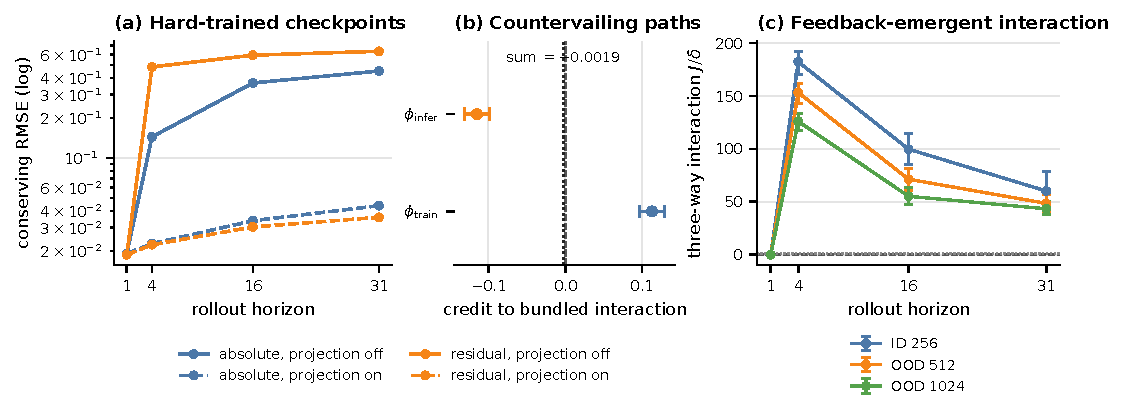
\includegraphics[width=\linewidth]{figures/pdebench_cube_mechanism.pdf}
  \caption{The projector becomes part of the learned autoregressive system. (a) At OOD 512,
  projected and unprojected hard-checkpoint evaluations agree in conserving RMSE at horizon one,
  as Proposition~\ref{prop:decoupling} requires, then diverge after feedback. Solid lines turn
  projection off; dashed lines retain it. (b) The primary path-averaged training and inference
  credits are large, opposite-signed, and sum to the small bundled interaction (vertical dotted
  line). (c) The three-way interaction, normalized by each cell's SESOI, is near zero at horizon
  one and material from horizon four at every resolution. Error bars are 95\% paired CIs.}
  \label{fig:cube}
\end{figure}

Consequently, $J=\CubeJ$ [\CubeJLow, \CubeJHigh] is \CubeJOverSesoi{} times the frozen
SESOI and passes the material-nonadditivity rule; its Holm-adjusted sign-flip $p$-value is
$\CubeHolmP$. All \CubeMaterialCells{} resolution cells at horizons 4, 16, and 31 are materially non-additive,
whereas none of the three horizon-one cells is. The path-averaged contributions
$\phi_{\mathrm{train}}=\CubePhiTrain$ and
$\phi_{\mathrm{infer}}=\CubePhiInfer$ are individually large and opposite-signed, leaving only
$I_{\mathrm{bundle}}=\CubeIBundle$ after cancellation. Thus the apparently benign deployed
comparison does not imply modularity. Proposition~\ref{prop:gauge} explains why hard training need
not determine a usable raw invariant channel; the horizon-one identity followed by divergence in
every registered horizon-four cell localizes the observed damage to autoregressive state feedback
after that gauge is exposed.

\subsection{The registered U-Net transfer does not pass its gate}

Replacing the FNO body with the frozen 66,941-parameter U-Net changes the boundary. Its ordinary
four-trained-cell interaction is nonzero,
$I_{\mathrm{bundle}}=\UNetIBundle$ [\UNetIBundleLow, \UNetIBundleHigh], but completing the cube
gives primary $J=\UNetJ$ [\UNetJLow, \UNetJHigh], classified \emph{\UNetClassification}.
Only \UNetMaterialCells/12 mandatory cells are materially non-additive, versus the registered
6/12 requirement, so the architecture-transfer gate \emph{\UNetAdmission}. All three material
cells are ID-256 at horizons 4, 16, and 31; selecting them after the unresolved OOD-512 primary
would reverse the prospective decision. Thus the FNO result is not architecture-general, and a
nonzero four-cell interaction does not by itself establish training--inference path dependence.

\subsection{Independent shallow water reproduces and amplifies the path dependence}

The prospectively frozen 2D shallow-water replication passes the same admission rule on a
different equation, dimension, boundary geometry, and linear mass invariant. Its ordinary
four-trained-cell interaction is \SWECoreInteraction{}
[\SWECoreInteractionLow, \SWECoreInteractionHigh]. Completing the cube instead gives
$J=\SWEJ$ [\SWEJLow, \SWEJHigh], whose magnitude is \SWEJOverSesoi{} times the frozen SESOI
(Holm $p=\SWEHolmP$). The interaction is practically additive at horizon one at both resolutions,
then material at horizons 4, 16, and 31, for \SWEMaterialCells/8 mandatory cells.

The diagnostic failure is sharply coordinate dependent: removing the projector from the
hard-trained absolute checkpoint raises mean conserving RMSE from \SWEAOneOne{} to
\SWEAOneZero{}, whereas the corresponding residual checkpoint remains near \SWEROneOne{} versus
\SWEROneZero{}. The path-averaged training and inference credits are again large and opposing,
\SWEPhiTrain{} and \SWEPhiInfer{}, summing to the much smaller bundled interaction. This is not a
claim that the unprojected hard model is a sensible deployment mode; it is evidence that the
projector is constitutive of what projected training learned.

The independent admissibility test does not reveal a hidden cost. At OOD-128/horizon-31, adding
projection to free-trained checkpoints improves maximum mass drift by \SWETradeoffConservation{}
[\SWETradeoffConservationLow, \SWETradeoffConservationHigh], conserving RMSE by
\SWETradeoffDynamics{} [\SWETradeoffDynamicsLow, \SWETradeoffDynamicsHigh], and mean negative-depth
deficit by \SWETradeoffPositivity{} [\SWETradeoffPositivityLow,
\SWETradeoffPositivityHigh]. Under the frozen sign convention and rule, this is a
\emph{\SWETradeoffClassification}, not a conservation--positivity trade-off.

\subsection{A direct intervention confirms gauge-to-dynamics feedback}

The two-step same-checkpoint intervention isolates the proposed feedback link rather than inferring
it from rollout timing. The first histories differ only by the raw prediction's uniform invariant
component; both then pass through the same compatible raw forward map. In the primary OOD-512
cell, the conserving-channel response has feedback RMSE \GaugeFeedbackRMSE{}
[\GaugeFeedbackRMSELow, \GaugeFeedbackRMSEHigh] and a feedback-to-projected-baseline ratio of
\GaugeRatio{} [\GaugeRatioLow, \GaugeRatioHigh]. The latter is \GaugeRatioOverThreshold{} times
the frozen 0.10 practical threshold and is classified as \emph{\GaugeClassification}.
All \GaugeMaterialCases/3 registered resolutions reach the same classification, and both absolute
and residual coordinates do so separately. The maximum numerical contamination is only
\GaugeMaxContamination{} of the projected baseline, below the prespecified
\GaugeContaminationLimit{} gate.

This establishes that an invariant-direction input perturbation can transfer directly into the
learned admissible dynamics. It does not show that the two-step magnitude ranks eventual rollout
failure across seeds: its Spearman association with coordinate-averaged horizon-16 removal harm is
$\rho=\GaugeAssociationRho$ [\GaugeAssociationRhoLow, \GaugeAssociationRhoHigh], classified
\emph{\GaugeAssociationClassification}. We therefore claim existence and materiality of the
feedback channel, not a seed-level quantitative explanation of every long-horizon divergence.

\paragraph{Local gradient boundary.}

The frozen first-minibatch intervention finds an absolute-minus-residual one-Adam-step effect of
$\CubeOneStepInteraction$ [$\CubeOneStepInteractionLow$,
$\CubeOneStepInteractionHigh$]. This rejects an exact local equality, but not the stronger
mechanism test. Its paired-seed association with the inference-matched final training interaction
$T_1=\CubeFinalTrainingInteraction$ is only $\rho=\CubeMechanismRho$ with 95\% bootstrap CI
[$\CubeMechanismRhoLow$, $\CubeMechanismRhoHigh$], yielding the prespecified classification
\emph{\CubeMechanismClassification}. The analogous bundled association is also unsupported.
We therefore do not claim that initial gradient alignment explains which seeds develop the final
effect. The direct input-gauge intervention establishes a material feedback channel; the gradient
diagnostic supplies a negative boundary on a competing local explanation.

\paragraph{Guarantee versus predictive attribution.}

Hard and projected rollouts satisfy the invariant while free models have no such guarantee.
Because conserving RMSE excludes the mechanically corrected channel and fixed projection cannot
change it (Proposition~\ref{prop:decoupling}), our accuracy result concerns training and feedback
through the projector, not a detachable post-hoc correction.

\section{Implications and conclusion}

\paragraph{Audit training and deployment jointly.}
A free absolute model versus a hard residual model estimates a bundled treatment; even four
trained cells omit deployment dependence. Add and remove projection on both free- and hard-trained
checkpoints while retaining weights, because retraining changes the intervention. The usual
asymmetric comparison---adding projection to a free checkpoint without removing it from a hard
one---cannot detect learned projector dependence.

\paragraph{Do not interpret raw outputs of a projected model as identified predictions.}
Because the hard loss is invariant along the projection gauge, raw hard-checkpoint values are
diagnostic latent quantities, not trained standalone forecasts. Model surgery, distillation,
quantization, or fallbacks that bypass a ``post-processing'' layer can therefore change dynamics.

\paragraph{Report orthogonal channels and failed mechanisms.}
Report both $\lVert Qe\rVert$ and $\lVert Pe\rVert$: total RMSE rewards mechanically deleted drift,
whereas conservation error alone hides admissible-direction damage. Nonlinear conditions such as
positivity remain separate (Proposition~\ref{prop:positivity}). The direct gauge response is
material, but neither its final-harm association nor the local-gradient association is supported.
The failed U-Net gate also prevents an architecture-general mechanism claim. Exact enforcement
should therefore be evaluated as part of the trained transition, not as a detachable correction.

\section{Limitations and non-claims}

Evidence spans two public datasets, one coefficient/scenario per equation, uniform mass, and
resolution shifts only; it does not cover nonlinear invariants, noise, or coefficient and
initial-condition shifts. Both positive PDE transfers use FNOs. The larger U-Net does not pass its
frozen gate and is not capacity matched, so architecture scope remains open. The shallow-water
surrogate observes depth but not momentum or velocity, making its evidence partial-state rather
than full-system fidelity. Projector removal is diagnostic, and gauge non-identification does not
force every optimizer to select an unstable representative. Credits, the training null, and the
10\% SESOI condition on the fixed design; cells share trained models, and intervals condition on
the frozen trajectories rather than every initial-condition distribution.

\subsection*{Reproducibility statement}

Appendix~\ref{app:protocol} records the data version, split, conservative restriction, model,
optimization, seeds, inference units, and frozen decision rules. The supplementary artifact
contains the Hydra configurations, immutable data-file and checkpoint locks, 450 core records, 270
zero-training cube records, 60 local-gradient records, 60 fresh direct-gauge records, validation
tests, one-shot analyzers, and the exact JSON used to generate every reported empirical estimate and
Figure~\ref{fig:cube}. Checkpoint-lock manifests bind all 360 final weight files by path, byte count,
payload identity, and SHA-256; this does not imply that the weight bytes are embedded in the PDF
supplement. The excluded 10-record numerical preflight is retained by hash but is never merged or
analyzed.
All formal records bind to source and protocol hashes.

\subsection*{AI use statement}

Generative AI tools were used to help formulate and critically revise the attribution framework,
mathematical statements and proof drafts, hypotheses and the prospective experiment protocol;
implement and test experiment and analysis code; prepare the conservative data interface; interpret
frozen outputs; discover and summarize related literature; generate figure code; format references;
and draft and edit the manuscript. They were not used to generate the underlying PDEBench
observations. The authors
reviewed the primary sources, executable tests, immutable hashes, analysis outputs, mathematical
claims, and all AI-assisted text and code. The authors take responsibility for the final content,
including claims and artifacts produced with AI assistance.

\bibliography{refs}
\bibliographystyle{iclr2027_conference}

\appendix

\section{Proof of projection decoupling}
\label{app:proof}

Because the target satisfies the invariant, $P(y-x)=0$. Therefore
\begin{align}
  \Pi_x(\hat y)-y
  &=\hat y-P(\hat y-x)-y \\
  &=e-P\bigl((\hat y-y)+(y-x)\bigr) \\
  &=e-Pe=Qe.
\end{align}
Applying $P$ gives zero and applying $Q$ returns $Qe$. Orthogonality of $P$ and $Q$ gives the
squared-error decomposition.

\section{Proof of the projected-training gauge}
\label{app:gauge}

Because $Pa=a$ for the rank-one projector onto $\operatorname{span}(a)$,
\begin{align}
  \Pi_x(z+\alpha a)
  &=z+\alpha a-P(z+\alpha a-x) \\
  &=z-P(z-x)+\alpha(a-Pa) \\
  &=\Pi_x(z).
\end{align}
Thus every realizable raw map in the equivalence class
$\{z+\alpha a:\alpha\colon\mathcal X\rightarrow\mathbb R\}$ induces exactly the same projected
prediction and loss. Projected observations cannot distinguish members of this class, so the raw
invariant-channel representative is unidentified without an additional restriction. This is an
output-space statement; shared parameters may still couple the identified and unidentified
channels, as analyzed by Propositions~\ref{prop:training-null} and \ref{prop:ntk-transfer}.

\section{Proof of conservation--positivity compatibility}
\label{app:positivity}

For $a=\mathbf{1}$, the projector subtracts the prediction's mean excess:
$\Pi_x(z)_i=z_i+m(x)-m(z)$. Therefore $\Pi_x(z)_i\geq0$ for every coordinate exactly when
$z_i\geq m(z)-m(x)$ for every coordinate, which is equivalent to
$\min_i z_i\geq m(z)-m(x)$. Taking any nonnegative $z$ with
$0\leq\min_i z_i<m(z)-m(x)$ proves that exact mass projection can create a negative component.

\section{Proof of the channel-separable training null}
\label{app:training-null}

For either coordinate choice, the conserving component of both the free and hard prediction is
$Q(b_s+z_Q(\theta_Q))$ because $Qz_P=0$. The free squared loss decomposes orthogonally into a term
depending only on $\theta_Q$ and a violating-channel term depending only on $\theta_P$; the hard
loss retains the first term and makes the second constant. The separable regularizer preserves
this equality of the $\theta_Q$ objectives. Thus paired minibatches give identical gradients for
$\theta_Q$ at every step. Equal initialization and a blockwise deterministic optimizer imply by
induction that all $\theta_Q$ iterates, and hence all conserving predictions, are identical. The
paired conserving-error difference is therefore zero.

\section{Proof of tangent-kernel channel transfer}
\label{app:ntk-transfer}

The two parameter displacements differ by
$\theta_F^+-\theta_H^+=-\eta g_P$. Because
$g_Q=J_\theta^\top\bar Qe$ and $g_P=J_\theta^\top\bar Pe$, the linearized conserving-output
difference is
\begin{equation}
  \bar QJ_\theta(\theta_F^+-\theta_H^+)
  =-\eta\bar QJ_\theta J_\theta^\top\bar Pe
  =-\eta\bar QK_\theta\bar Pe.
\end{equation}
The inner-product identity follows from
$g_Q^\top g_P=(\bar Qe)^\top J_\theta J_\theta^\top(\bar Pe)$.
If $\bar QK_\theta\bar P=0$, the first expression vanishes for every violating residual.
Conversely, vanishing for every vector in the range of $\bar P$ implies
$\bar QK_\theta\bar P=0$.

\section{Proof of the one-step gradient-coupling bound}
\label{app:gradient-coupling}

For a function with $\beta$-Lipschitz gradient, the descent lemma gives
$L_Q(\theta+u)=L_Q(\theta)+g_Q^\top u+r_u$ with
$|r_u|\leq \beta\lVert u\rVert_2^2/2$. Apply it to
$u=-\eta(g_Q+g_P)$ and $v=-\eta g_Q$, then subtract the two expansions. Their linear terms differ
by $-\eta g_Q^\top g_P$ and the triangle inequality gives
\begin{equation}
  |r_u-r_v|\leq \frac{\beta\eta^2}{2}
  \left(\lVert g_Q+g_P\rVert_2^2+\lVert g_Q\rVert_2^2\right),
\end{equation}
which is Equation~\ref{eq:gradient-coupling}.

\section{Proof of three-cell non-identification}
\label{app:missing-cell}

Fix arbitrary nonnegative observed values $Y_{A0}$, $Y_{R0}$, and $Y_{R1}$, and let
$C=Y_{A0}-Y_{R0}+Y_{R1}$. For any $c\leq C$, choose
\begin{equation}
  Y_{A1}=Y_{A0}-Y_{R0}+Y_{R1}-c.
\end{equation}
This value is nonnegative, and substitution into Equation~\ref{eq:interaction} gives
$\Ipath=c$ while leaving every observed cell unchanged. The half-line $c\leq C$ contains
infinitely many choices. Because both $P_1=Y_{A1}-Y_{R1}$ and
$E_A=Y_{A0}-Y_{A1}$ depend on this unobserved value, the Shapley credits in
Equation~\ref{eq:shapley} are also unidentified. Proposition
\ref{prop:decoupling} constrains the conserving error of a fixed projected prediction, not the
parameters learned by training through the hard absolute-output layer, so projection cannot supply
the missing intervention.

\clearpage
\section{Complete frozen intervention-cube summary}
\label{app:cells}

Table~\ref{tab:allcells} lists the three-way interaction in every mandatory
resolution--horizon cell. It is not a set of twelve replications: all rows reuse the same paired
checkpoints, and Holm correction is applied to their sign-flip tests. The frozen ordered
classification uses each cell's own $\delta=0.1\overline{Y}_{R00}$.

\begin{table}[H]
  \caption{All mandatory PDEBench Advection intervention-cube cells. $J/\delta$ gives effect size
  relative to the prespecified practical threshold; $p$ is Holm-adjusted.}
  \label{tab:allcells}
  \centering
  \scriptsize
  \resizebox{\textwidth}{!}{%
  \begin{tabular}{llrrrll}
    \toprule
    Case & Horizon & $J$ & 95\% CI & $J/\delta$ & Class & Holm $p$ \\
    \midrule
    ID 256 & 1 & $2.52\!\times\!10^{-10}$ & [$4.29\!\times\!10^{-11}$, $4.76\!\times\!10^{-10}$] & 0.0 & smaller & 0.0932 \\
ID 256 & 4 & 0.3256 & [0.3041, 0.3434] & 182.2 & material & 0.0001 \\
ID 256 & 16 & 0.2205 & [0.1893, 0.2522] & 99.8 & material & 0.0001 \\
ID 256 & 31 & 0.1667 & [0.1162, 0.2175] & 60.2 & material & 0.0001 \\
OOD 512 & 1 & $1.10\!\times\!10^{-10}$ & [$-1.96\!\times\!10^{-10}$, $4.10\!\times\!10^{-10}$] & 0.0 & additive & 0.7632 \\
OOD 512 & 4 & 0.3397 & [0.3164, 0.3593] & 153.2 & material & 0.0001 \\
OOD 512 & 16 & 0.2297 & [0.1964, 0.2634] & 71.4 & material & 0.0001 \\
OOD 512 & 31 & 0.1914 & [0.1612, 0.2237] & 48.5 & material & 0.0001 \\
OOD 1024 & 1 & $-1.24\!\times\!10^{-10}$ & [$-3.89\!\times\!10^{-10}$, $1.48\!\times\!10^{-10}$] & 0.0 & additive & 0.7632 \\
OOD 1024 & 4 & 0.3450 & [0.3209, 0.3651] & 126.0 & material & 0.0001 \\
OOD 1024 & 16 & 0.2338 & [0.2004, 0.2676] & 55.3 & material & 0.0001 \\
OOD 1024 & 31 & 0.2203 & [0.1913, 0.2531] & 43.4 & material & 0.0001 \\
\bottomrule

  \end{tabular}}
\end{table}

\section{Primary eight cells and artifact identity}
\label{app:protocol}

Table~\ref{tab:eight-cells} makes the full primary intervention transparent. Training and inference
projection are separate binary factors. The four off-diagonal inference cells reuse locked weights
and take zero optimizer steps.

\begin{table}[H]
  \caption{Mean conserving RMSE in all eight OOD-512, horizon-16 cells across 30 paired seeds.}
  \label{tab:eight-cells}
  \centering
  \small
  \begin{tabular}{llrr}
    \toprule
    Training & Inference & Absolute & Residual \\
    \midrule
    free & projector off & \CubeAZeroZero & \CubeRZeroZero \\
    free & projector on  & \CubeAZeroOne & \CubeRZeroOne \\
    hard & projector off & \CubeAOneZero & \CubeROneZero \\
    hard & projector on  & \CubeAOneOne & \CubeROneOne \\
    \bottomrule
  \end{tabular}
\end{table}

For reference, the primary conserving-RMSE means are \FactorAZero{} for \texttt{free},
\FactorRZero{} for \texttt{free\_res}, \FactorAOne{} for \texttt{hard\_abs}, \FactorROne{} for
\texttt{hard}, and \FactorProjected{} for free-trained \texttt{projection}. These descriptive
quantities do not define extra hypothesis tests. A projection rollout feeds corrected states back
into the FNO, so after its first step its inputs differ from an unprojected rollout; the fixed-input
identity is checked at horizon one rather than assumed at horizon 16.

The dataset is DaRUS PDEBench version 8, file ID 255674,
\texttt{1D\_Advection\_Sols\_beta0.4.hdf5}, released under CC BY 4.0. The observed file size is
8,232,966,952 bytes. Its content hashes are
\path{MD5:d595bbfd2c659df995a93cd40d6ea568} and
\path{SHA256:d973ff2bb3c2a5edf42957ff029b78672451532ebd6bf475848ff23cfd3ee3b6}.
The fresh core JSONL/analysis SHA-256 prefixes are
\path{d0c8257af992}/\path{15ab5898699e}; the zero-training cube prefixes are
\path{bee99e1b15d0}/\path{d12dc6d088d2}; and the local-diagnostic prefixes are
\path{fd5251a63f6d}/\path{e6edc0803477}. The direct-gauge rerun/analysis prefixes are
\path{285ba66aeb84}/\path{87ed9676386e}; its excluded 10-record numerical preflight is retained at
\path{f55983ec19d2}. The supplementary manifest records and verifies the complete hashes rather
than these display prefixes.

The inference unit is a seed, not a trajectory or rollout frame. All mechanisms within a seed use
the same training subset, deterministic window cycle, minibatch order, initialization tensor, and
evaluation trajectories. No model outcome was read before complete coverage and the integrity
gates passed. The failed v1 data-admission attempt used point decimation, produced no model record,
and was replaced prospectively by the exact block-average restriction used here.

\section{Registered U-Net architecture-transfer boundary}
\label{app:unet-artifacts}

Table~\ref{tab:unet-allcells} reports the complete mandatory transfer grid rather than only the
three favorable ID rows. The gate required both a material OOD-512/horizon-16 primary and at least
6/12 material cells. The primary is \emph{\UNetClassification}, and only
\UNetMaterialCells/12 cells are material, so the registered transfer \emph{\UNetAdmission}.
Six cells show smaller statistical non-additivity, one is practically additive, and two are
unresolved. This pattern is a boundary result, not evidence of absence in every U-Net cell.

\begin{table}[H]
  \caption{All mandatory U-Net intervention-cube cells. $J/\delta$ uses the same prespecified
  practical threshold as the FNO audit; $p$ is Holm-adjusted.}
  \label{tab:unet-allcells}
  \centering
  \scriptsize
  \resizebox{\textwidth}{!}{%
  \begin{tabular}{llrrrll}
    \toprule
    Case & Horizon & $J$ & 95\% CI & $J/\delta$ & Class & Holm $p$ \\
    \midrule
    ID 256 & 1 & $2.21\!\times\!10^{-10}$ & [$8.98\!\times\!10^{-12}$, $4.26\!\times\!10^{-10}$] & 0.0 & smaller & 0.2483 \\
ID 256 & 4 & -0.0791 & [-0.1135, -0.0428] & -27.3 & material & 0.0018 \\
ID 256 & 16 & 0.4236 & [0.2522, 0.6406] & 26.5 & material & 0.0002 \\
ID 256 & 31 & 0.8233 & [0.5034, 1.2144] & 23.1 & material & 0.0001 \\
OOD 512 & 1 & $-5.99\!\times\!10^{-10}$ & [$-1.15\!\times\!10^{-9}$, $-3.44\!\times\!10^{-11}$] & 0.0 & smaller & 0.2483 \\
OOD 512 & 4 & -0.0469 & [-0.0619, -0.0322] & -1.0 & smaller & 0.0001 \\
OOD 512 & 16 & -0.0841 & [-0.2666, 0.1333] & -0.6 & unresolved & 1.0000 \\
OOD 512 & 31 & -0.0188 & [-0.3469, 0.3441] & -0.1 & unresolved & 1.0000 \\
OOD 1024 & 1 & $2.86\!\times\!10^{-10}$ & [$-4.69\!\times\!10^{-10}$, $1.08\!\times\!10^{-9}$] & 0.0 & additive & 1.0000 \\
OOD 1024 & 4 & -0.0537 & [-0.0723, -0.0342] & -0.8 & smaller & 0.0002 \\
OOD 1024 & 16 & -0.3506 & [-0.5808, -0.0727] & -1.6 & smaller & 0.0747 \\
OOD 1024 & 31 & -0.6128 & [-1.1199, -0.0811] & -1.7 & smaller & 0.1933 \\
\bottomrule

  \end{tabular}}
\end{table}

\begin{table}[H]
  \caption{Mean U-Net conserving RMSE in the eight primary OOD-512, horizon-16 cells across 30
  paired seeds. Off-diagonal inference cells reuse locked weights and take zero optimizer steps.}
  \label{tab:unet-eight}
  \centering
  \small
  \begin{tabular}{llrr}
    \toprule
    Training & Inference & Absolute & Residual \\
    \midrule
    free & projector off & \UNetAZeroZero & \UNetRZeroZero \\
    free & projector on  & \UNetAZeroOne  & \UNetRZeroOne  \\
    hard & projector off & \UNetAOneZero  & \UNetROneZero  \\
    hard & projector on  & \UNetAOneOne   & \UNetROneOne   \\
    \bottomrule
  \end{tabular}
\end{table}

The U-Net merged core/analysis SHA-256 prefixes are
\texttt{\UNetCoreSHA}/\texttt{\UNetCoreAnalysisSHA}; the 120-checkpoint lock is
\texttt{\UNetLockSHA}; and the cube/analysis prefixes are
\texttt{\UNetCubeSHA}/\texttt{\UNetCubeAnalysisSHA}. The formal seeds are 7000--7029. Both fixed
15-seed workers exited before the core analyzer ran; the cube followed only after exact 150-record
coverage and checkpoint-lock verification. The supplementary manifest records the full hashes.

\section{Independent shallow-water artifact identity}
\label{app:swe-artifacts}

\begin{table}[H]
  \caption{All eight shallow-water primary OOD-128, horizon-16 cells. Entries are mean conserving
  RMSE across 30 paired seeds; off-diagonal cells change only the inference forward map of a
  locked checkpoint and take zero optimizer steps.}
  \label{tab:swe-eight}
  \centering
  \small
  \begin{tabular}{llrr}
    \toprule
    Training & Inference & Absolute & Residual \\
    \midrule
    free & projector off & \SWEAZeroZero & \SWERZeroZero \\
    free & projector on  & \SWEAZeroOne  & \SWERZeroOne  \\
    hard & projector off & \SWEAOneZero  & \SWEROneZero  \\
    hard & projector on  & \SWEAOneOne   & \SWEROneOne   \\
    \bottomrule
  \end{tabular}
\end{table}

The replication uses DaRUS PDEBench version 8, file ID 133021,
\texttt{2D\_rdb\_NA\_NA.h5}, with 6,626,098,972 bytes and hashes
\path{MD5:75d838c47aa410694bdc912ea7f22282} and
\path{SHA256:28f0c33723d70eebb420fc170e94b675c18e032fb697dcef080e114ca9645e3a}.
The data gate verifies all 1,000 group names, tensor and coordinate schemas, finiteness, strict
target positivity, mass drift, and both block-average restrictions. The merged core JSONL/analysis
SHA-256 prefixes are \path{5e486167a2a8}/\path{d194df9d3f8d}; the checkpoint lock prefix is
\path{772c52f9dbaa}; and the zero-training cube/analysis prefixes are
\path{69dfa936fd83}/\path{f8492362b377}. Exact hashes and the outcome-blind numerical-analysis
amendment are retained in the supplementary manifest. The amendment changes only the tolerance
for comparing algebraically identical floating-point rearrangements; it does not alter any cell,
effect, interval, threshold, or classification.

\section{Registered public-data stops with zero model records}
\label{app:data-stops}

Two other prospectively registered PDEBench blocks stopped at their frozen data contracts and do
not enter any estimate. The periodic 1D Burgers file passed its byte count, MD5, and SHA-256 checks
but failed the registered spatial-coordinate start before solution-tensor values were read. The
compressible Navier--Stokes file likewise passed transport hashes but exposed 102 time coordinates
rather than the frozen 101 before field-value scanning. We did not amend either schema after the
failure: no data lock, model preflight, model record, or model metric was produced. The terminal
decisions and available admission log are retained in the artifact. These are data-contract stops,
not unfavorable replication outcomes.

\section{Separate synthetic stress test}
\label{app:synthetic}

A separately locked synthetic confirmation used seeds 1000--1029 and pilot-selected cells. It is
not pooled with PDEBench because its systems have different scales and its comparisons are not a
fully crossed factorial. \SyntheticSystems{} of ten prespecified systems completed with exactly
1,830 finite,
provenance-bound records. The A- and B-family synthetic Burgers jobs instead produced non-finite
outputs before a valid record could be serialized; their zero-record incidents were preserved and
excluded rather than repaired after outcomes.

Table~\ref{tab:synthetic} reports every completed system at its family-specific primary OOD case
and horizon one. The 95\% parameterization interval excludes zero in
\SyntheticParameterizationNonzero/\SyntheticSystems{} systems and all
\SyntheticParameterizationHolm{} paired tests remain significant after Holm correction, but
residual coordinates are favored in only \SyntheticResidualFavored/\SyntheticSystems; C-ad2d and
strong contraction favor absolute coordinates. Hard versus residual-free training is practically
equivalent under the frozen 10\% SESOI in \SyntheticEquivalent/\SyntheticSystems{} systems. Only
\SyntheticFullPass{} system (M2) satisfies the entire legacy conjunction, chiefly because
the 5\% ID/compute-overlap gate fails for at least one contrast in the other systems. This block
therefore supports neither a universal residual advantage nor a broad legacy-rule headline. Its
role is boundary evidence for why the public fully crossed interaction is needed.

\begin{table}[H]
  \caption{Separate synthetic stress test. $\Delta_P$ is free minus free-res conserving RMSE
  (95\% CI); positive values favor residual coordinates. $\Delta_E$ is free-res minus hard
  (90\% CI); positive values favor hard enforcement. ``Eq.'' is frozen hard/free-res
  equivalence, ``Overlap'' requires both ID/compute gates, and ``Full'' is the complete legacy
  conjunction. Effects are not comparable in magnitude across systems.}
  \label{tab:synthetic}
  \centering
  \scriptsize
  \resizebox{\textwidth}{!}{%
  \begin{tabular}{lrrrccc}
    \toprule
    System & $\Delta_P$ [95\% CI] & Holm $p$ & $\Delta_E$ [90\% CI] & Eq. & Overlap & Full \\
    \midrule
    A advection & 1.0749 [1.0705, 1.0792] & 2.91e-57 & -3.17e-5 [-1.94e-4, 1.33e-4] & yes & no & no \\
A diffusion & 1.1129 [1.1089, 1.1168] & 8.36e-59 & 3.15e-4 [1.30e-4, 5.06e-4] & yes & no & no \\
B advection & 1.0248 [0.9938, 1.0557] & 2.08e-32 & 0.0030 [-0.0020, 0.0080] & no & no & no \\
B diffusion & 0.8394 [0.8144, 0.8637] & 1.23e-32 & 5.03e-4 [1.26e-4, 8.80e-4] & no & no & no \\
C ad2d & -1.2089 [-1.2130, -1.2046] & 5.97e-59 & -6.12e-4 [-0.0054, 0.0047] & yes & no & no \\
H near & 0.9975 [0.9938, 1.0012] & 2.55e-58 & -1.24e-6 [-4.74e-6, 2.24e-6] & yes & no & no \\
H strong & -1.0941 [-1.1156, -1.0680] & 2.80e-36 & 5.27e-6 [-3.46e-6, 1.42e-5] & yes & no & no \\
M2 FIFO & 0.0048 [0.0041, 0.0055] & 7.30e-14 & 1.66e-4 [-1.37e-4, 4.86e-4] & yes & yes & yes \\
\bottomrule

  \end{tabular}}
\end{table}

\end{document}
